\documentclass{ximera}
%%% You can put user macros here
%% However, you cannot make new environments

\listfiles

\graphicspath{{./}{firstExample/}{secondExample/}}

\usepackage{tikz}
\usepackage{tkz-euclide}
\usepackage{tikz-3dplot}
\usepackage{tikz-cd}
\usetikzlibrary{shapes.geometric}
\usetikzlibrary{arrows}
%\usetkzobj{all}
\pgfplotsset{compat=1.13} % prevents compile error.

%\renewcommand{\vec}[1]{\mathbf{#1}}
\renewcommand{\vec}{\mathbf}
\newcommand{\RR}{\mathbb{R}}
\newcommand{\dfn}{\textit}
\newcommand{\dotp}{\cdot}
\newcommand{\id}{\text{id}}
\newcommand\norm[1]{\left\lVert#1\right\rVert}
 
\newtheorem{general}{Generalization}
\newtheorem{initprob}{Exploration Problem}

\tikzstyle geometryDiagrams=[ultra thick,color=blue!50!black]

%\DefineVerbatimEnvironment{octave}{Verbatim}{numbers=left,frame=lines,label=Octave,labelposition=topline}



\usepackage{mathtools}


\author{Anna Davis} \title{MTH 140 Test 2} 

\begin{document}

\begin{abstract}

\end{abstract}
\maketitle
 \textit{You have 1 hour and 20 minutes to complete this test.  Each answer is worth 1 point.}
\begin{problem}\label{prob:exam2prob1}
The diagram below shows two spinners.  Two spinners are spun and the values are added together.  Let $X$ be the sum of the values.  

\begin{image}
   
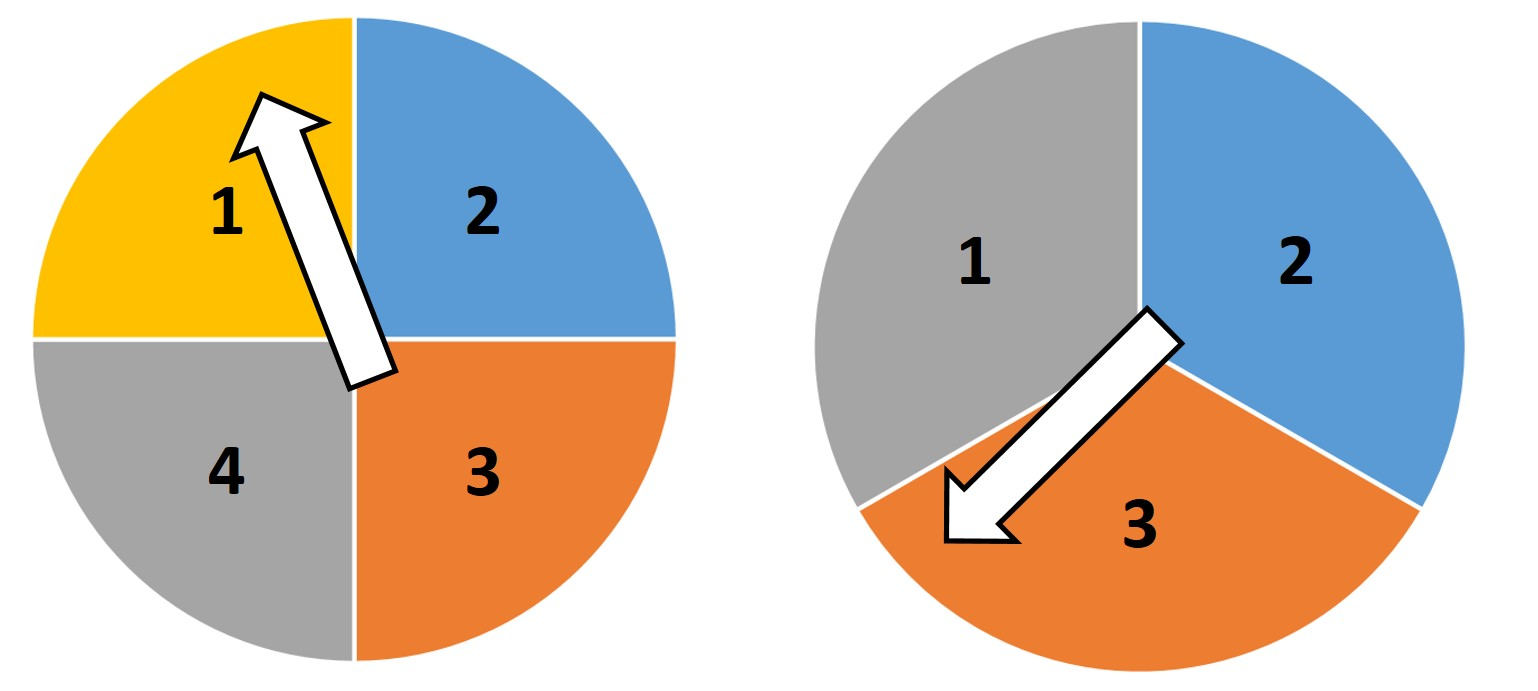
\includegraphics[height=1in]{test2spinners.jpg}
 
\end{image}



\begin{enumerate}
    \item Fill out the following table to help you determine probabilities of obtaining various sums.
    
\begin{center}
\begin{tabular}{|c|c|c|c|}
 \hline
 && &   \\
 & $1$& $2$ &$3$ \\
 && &   \\
  \hline
  && & \\
 $1$&$\answer{2}$&$\answer{3}$&$\answer{4}$ \\
  &&& \\
 \hline
  &&& \\
 $2$&$\answer{3}$&$\answer{4}$ &$\answer{5}$ \\
  &&& \\
 \hline
  &&& \\
  $3$&$\answer{4}$&$\answer{5}$  &$\answer{6}$ \\
  &&& \\
 \hline
 &&& \\
  $4$&$\answer{5}$&$\answer{6}$  &$\answer{7}$ \\
  &&& \\
 \hline
 \end{tabular}
\end{center}    
    
    
\item $$P(1)=\answer{0}$$ $$P(2)=\answer[tolerance=0.01]{\frac{1}{12}}$$ $$P(5)=\answer[tolerance=0.01]{\frac{1}{4}}$$ $$P(x<6)=\answer{\frac{9}{12}}$$ $$P(x>2)=\answer[tolerance=0.01]{\frac{11}{12}}$$


\item Fill out the table provided below and find the expected value $(\mu)$ and the standard deviation $(\sigma)$.

\begin{center}
\begin{tabular}{|c|c|c|c|}
 \hline
 && &   \\
 Sum of Values ($x$) & $P(x)$& $xP(x)$ &$(x-\mu)^2P(x)$ \\
 && &   \\
  \hline
  && & \\
 \quad$2$\quad&$\answer[tolerance=0.01]{\frac{1}{12}}$&$\answer[tolerance=0.01]{\frac{1}{6}}$&$\answer[tolerance=0.01]{0.521}$ \\
  &&& \\
 \hline
  &&& \\
 \quad $3$&$\answer[tolerance=0.01]{\frac{2}{12}}$&$\answer[tolerance=0.01]{\frac{1}{2}}$ & $\answer[tolerance=0.01]{0.375}$ \\
  &&& \\
 \hline
  &&& \\
  \quad $4$&$\answer[tolerance=0.01]{\frac{1}{4}}$& $\answer[tolerance=0.01]{1}$ &$\answer[tolerance=0.01]{0.0625}$ \\
  &&& \\
 \hline
  & &&\\
 \quad $5$& $\answer[tolerance=0.01]{\frac{1}{4}}$&$\answer[tolerance=0.01]{\frac{5}{4}}$  & $\answer[tolerance=0.01]{0.0625}$\\
  &&&\\
 \hline
  & &&\\
 \quad $6$&$\answer[tolerance=0.01]{\frac{1}{6}}$ & $\answer[tolerance=0.01]{1}$ & $\answer[tolerance=0.01]{0.375}$\\
  &&&\\
 \hline
 & &&\\
 \quad $7$&$\answer[tolerance=0.01]{\frac{1}{12}}$ & $\answer[tolerance=0.01]{\frac{7}{12}}$ & $\answer[tolerance=0.01]{0.521}$\\
  &&&\\
 \hline
\end{tabular}
\end{center}
\vskip 0.5in
$$\mu=\answer{4.5};\quad \sigma =\answer[tolerance=0.01]{1.38}$$
\end{enumerate}

\end{problem}

\begin{problem}\label{prob:exam2prob2}
Suppose the graph below represents a continuous probability distribution function.
\begin{image}
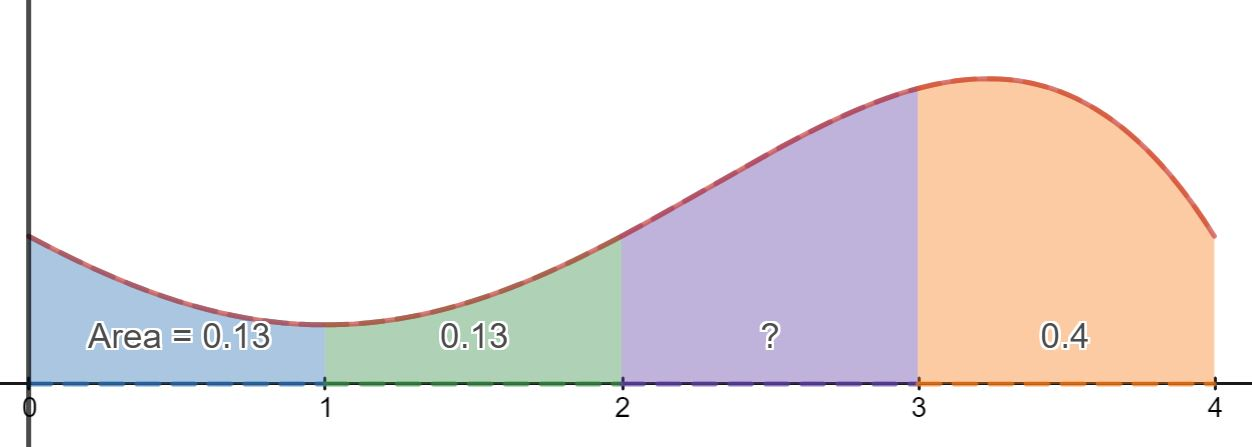
\includegraphics{test2pic3.JPG}
\end{image}
  \begin{enumerate}
      \item The missing area is: $\answer{0.34}$
      \item 
      
          $$P(1\leq x\leq 2)=\answer{0.13}$$
  
          $$P(x=1)=\answer{0}$$
   
          $$P(x>3)=\answer{0.4}$$
    
     
  \end{enumerate}
\end{problem}

\begin{problem}\label{prob:exam2prob3}
Use Geogebra to find the shaded area under the Standard Normal Curve, if the $z$-scores are marked. \begin{image}
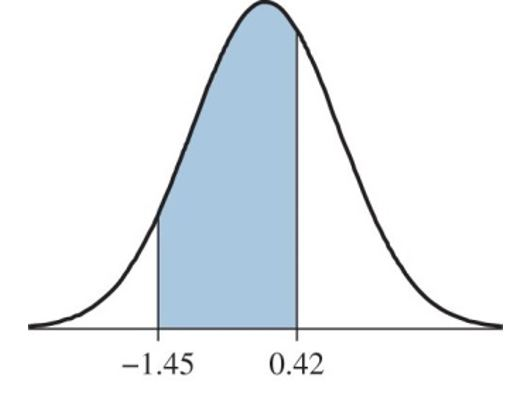
\includegraphics{test2pic2.JPG}
\end{image}

Shaded area (to four decimal places): $\answer[tolerance=0.0001]{0.5892}$
\end{problem}

\begin{problem}\label{prob:exam2prob4}
A company wants to evaluate its attrition rate, in other words, how long new hires stay with the company. Let $X$ be the number of years a new hire will stay with the company.
Let $P(x)$ be the probability that a new hire will stay with the company $x$ years.  Over the years, they have established the following probability
distribution.  Find the missing value in the table.
\begin{center}
\begin{tabular}{|c|c|}
 \hline
 & \\
 $x$&$P(x)$\\
 & \\
 \hline
  & \\
 $0$&$0.12$\\
 & \\
 \hline
 & \\
 $1$&$0.18$\\
 & \\
 \hline
  & \\
 $2$&$0.30$\\
 & \\
 \hline
  & \\
 $3$&$0.15$\\
 & \\
 \hline
  & \\
 $4$&$\answer{0.1}$\\
 & \\
 \hline
  & \\
 $5$&$0.10$\\
 & \\
 \hline
  & \\
 $6$&$0.05$\\
 & \\
 \hline
\end{tabular}
\end{center}
Find the probability:
$$P(x\geq 5)=\answer{0.15}$$

\end{problem}

\begin{problem}\label{prob:exam2prob5}
Suppose wait times at a bus stop are uniformly distributed and range from 0 minutes to 10 minutes.  The graph of the probability distribution function is shown below.
\begin{image}
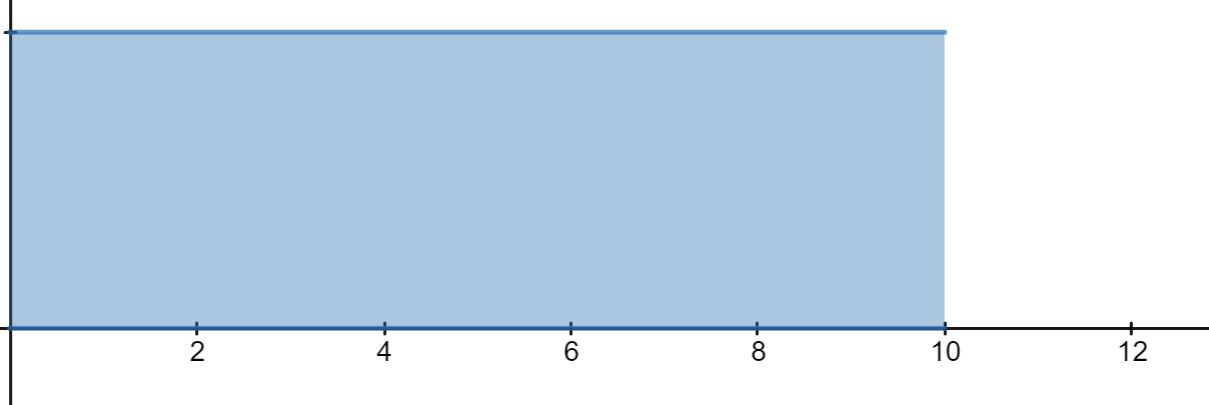
\includegraphics{test2waittime.JPG}
\end{image}
\begin{enumerate}
    \item The height of the rectangle is: $\answer{0.1}$
    \item 
    $$P(2<x<8)=\answer{0.6}$$
    \item 
    The mean waiting time is: $\answer{5}$ minutes.
\end{enumerate}
\end{problem}

\begin{problem}\label{prob:exam2prob6}
Find the $z$-score for the $90$th percentile.  (Round to four decimal places.)
\begin{image}
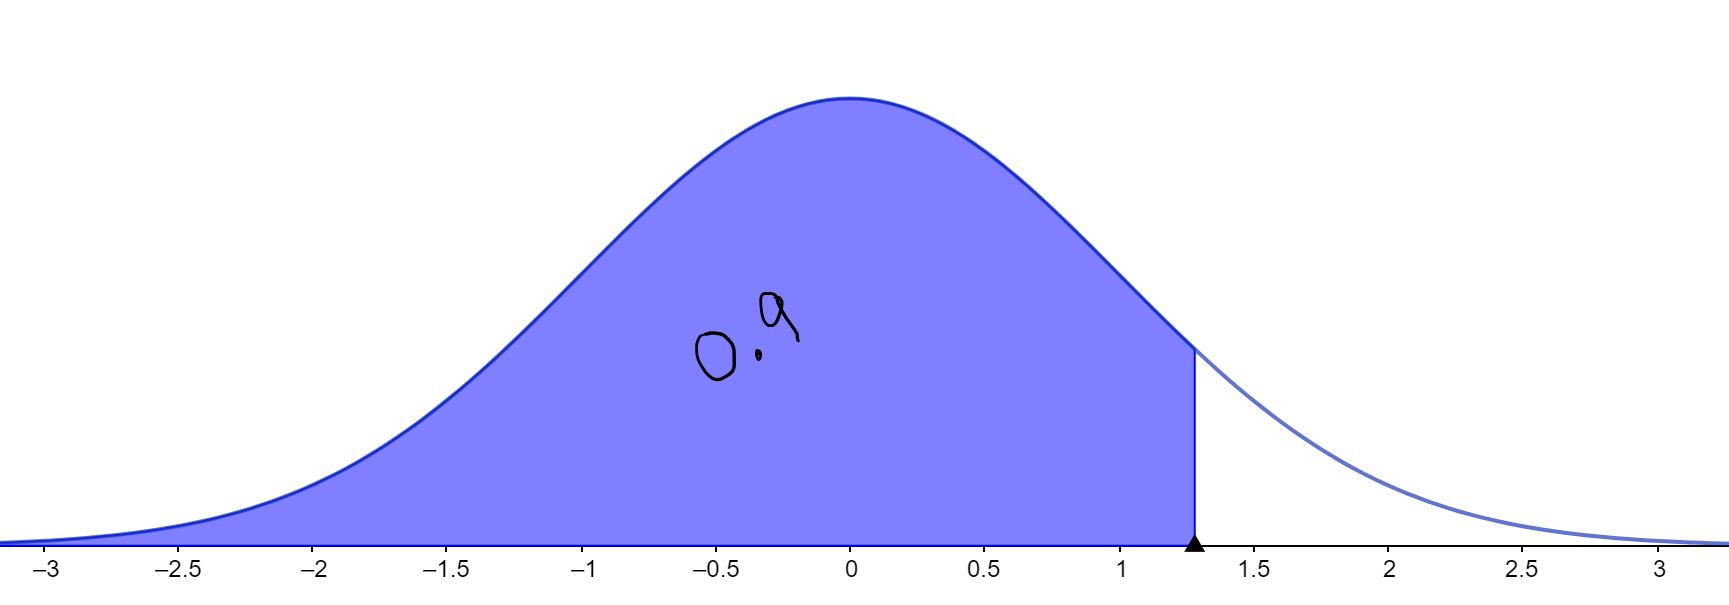
\includegraphics{test290thpercentile.JPG}
\end{image}
$$z=\answer[tolerance=0.0001]{1.2816}$$
\end{problem}

\begin{problem}\label{prob:exam2prob7}
The patient recovery time from a particular surgical
procedure is normally distributed with a mean of 5.3 days and a standard deviation of 2.1 days.  

The $90^{th}$ percentile for recovery time is $\answer{8}$ days. (Round to the nearest integer.)
\end{problem}

\begin{problem}\label{prob:exam2prob8}
Suppose test completion times for students taking an Intro to Sociology course at a large university have a mean of 44 minutes and standard deviation of 8 minutes.  Give an numeric answer for questions that can be answered.  Enter $na$ for questions that cannot be answered meaningfully.
\begin{enumerate}
\item The probability that a single student finished the test in less than 40 minutes is $\answer{na}$.
\item The probability that 40 students selected at random will have an average test completion time greater than 45 minutes is $\answer[tolerance=0.001]{0.2148}$.
\item The probability that 40 students selected at random will have an average test completion time between 40 and 42 minutes is $\answer[tolerance=0.001]{0.0563}$.
\end{enumerate}
\end{problem}
\end{document} 